
\documentclass{beamer}
\usecolortheme{dove}
\setbeamertemplate{navigation symbols}{}
\usepackage{amsmath,amssymb,amsfonts,amsthm, multicol, subfigure, color}
\usepackage{bm}
\usepackage{graphicx}
\usepackage{tabularx}
\usepackage{booktabs}
\usepackage{hyperref}
\usepackage{pdfpages}
\usepackage{xcolor}
\definecolor{seagreen}{RGB}{46, 139, 87}
\definecolor{mustard}{RGB}{234, 170, 0}
\def\independenT#1#2{\mathrel{\rlap{$#1#2$}\mkern2mu{#1#2}}}
\newcommand\indep{\protect\mathpalette{\protect\independenT}{\perp}}
\def\log{\text{log}}
\newcommand\logit{\text{logit}}
\newcommand\iid{\stackrel{\text{iid}}{\sim}}
\newcommand\E{\text{E}}
\newcommand\V{\text{V}}
\renewcommand\P{\text{P}}
\newcommand{\Cov}{\text{Cov}}
\newcommand{\Cor}{\text{Cor}}
\newcommand\doop{\texttt{do}}
\usepackage{stackrel}
\usepackage{tikz}
\usetikzlibrary{arrows,shapes.arrows,positioning,shapes,patterns,calc}
\newcommand\slideref[1]{\vskip .1cm \tiny \textcolor{gray}{{#1}}}
\newcommand\red[1]{\color{red}#1}
\newcommand\blue[1]{\color{blue}#1}
\newcommand\gray[1]{\color{gray}#1}
\newcommand\seagreen[1]{\color{seagreen}#1}
\newcommand\purple[1]{\color{purple}#1}
\newcommand\orange[1]{\color{orange}#1}
\newcommand\black[1]{\color{black}#1}
\newcommand\white[1]{\color{white}#1}
\newcommand\teal[1]{\color{teal}#1}
\newcommand\magenta[1]{\color{magenta}#1}
\newcommand\Fuchsia[1]{\color{Fuchsia}#1}
\newcommand\BlueGreen[1]{\color{BlueGreen}#1}
\newcommand\bblue[1]{\textcolor{blue}{\textbf{#1}}}
\newcommand\bred[1]{\textcolor{red}{\textbf{#1}}}
\newcommand\bgray[1]{\textcolor{gray}{\textbf{#1}}}
\newcommand\bgreen[1]{\textcolor{seagreen}{\textbf{#1}}}
\newcommand\bref[2]{\href{#1}{\color{blue}{#2}}}
\colorlet{lightgray}{gray!40}
\pgfdeclarelayer{bg}    % declare background layer for tikz
\pgfsetlayers{bg,main} % order layers for tikz
\newcommand\mycite[1]{\begin{scriptsize}\textcolor{darkgray}{(#1)}\end{scriptsize}}
\newcommand{\tcframe}{\frame{
%\small{
\only<1|handout:0>{\tableofcontents}
\only<2|handout:1>{\tableofcontents[currentsubsection]}}
%}
}

\newcommand{\goalsframe}{\begin{frame}{Learning goals for today}
By the end of class, you will be able to
\begin{itemize}
    \item conceptually trace the origins of racial wealth inequality to explicitly racist policies
    \item map racial segregation in a city of your choosing
\end{itemize} \vskip .2in
\end{frame}}

\usepackage[round]{natbib}
\bibliographystyle{humannat-mod}
\setbeamertemplate{enumerate items}[default]
\usepackage{mathtools}

\title{Studying Social Inequality with Data Science}
\author{Ian Lundberg}
\date{\today}

\begin{document}

\begin{frame}
\begin{tikzpicture}[x = \textwidth, y = \textheight]
\node at (0,0) {};
\node at (1,1) {};
\node[anchor = north west, align = left, font = \huge] at (0,.9) {Studying\\Social Inequality\\with Data Science};
\node[anchor = north east, align = right] (number) at (1,.9) {INFO 3370 / 5371\\Spring 2023};
\node[anchor = north, font = \Large, align = left] at (.5,.5) {\bblue{Reparations: Case study}\\A Southern California beach is\\returned to Black owners};
\end{tikzpicture}
\end{frame}

%\goalsframe

\begin{frame}
\begin{tikzpicture}[x = \textwidth, y = \textheight]
\node[anchor = north west] at (0,1) {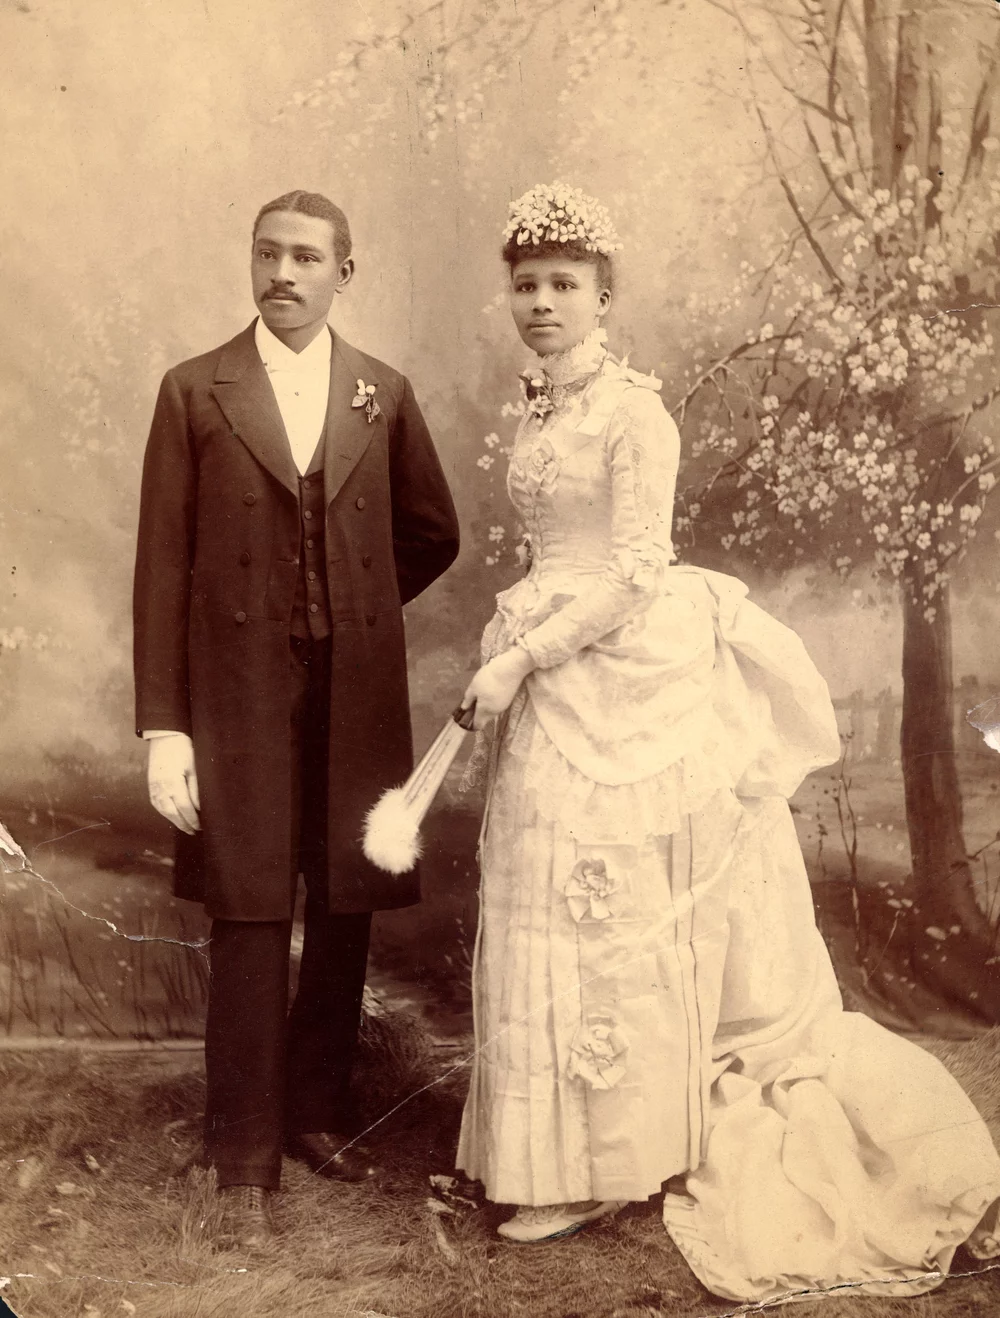
\includegraphics[height = \textheight]{figures/bruces}};
\node[anchor = south east, align = right] at (1,0) {Source:\\California African\\American Museum\\via \href{https://www.npr.org/2021/10/10/1043821492/black-americans-land-history}{NPR}};
\end{tikzpicture}
\end{frame}

\begin{frame}
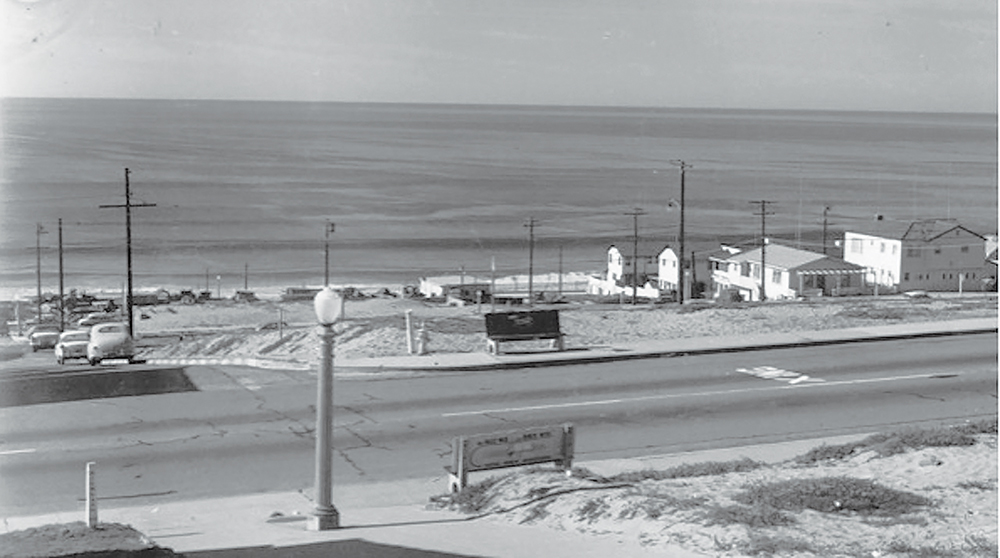
\includegraphics[width = \textwidth]{figures/bruces-beach-1950} \\
Source: Manhattan Beach Historical Society via \href{https://easyreadernews.com/bruces-beach-manhattan-beach-dispossession/}{Easy Reader News}
\end{frame}

\begin{frame}
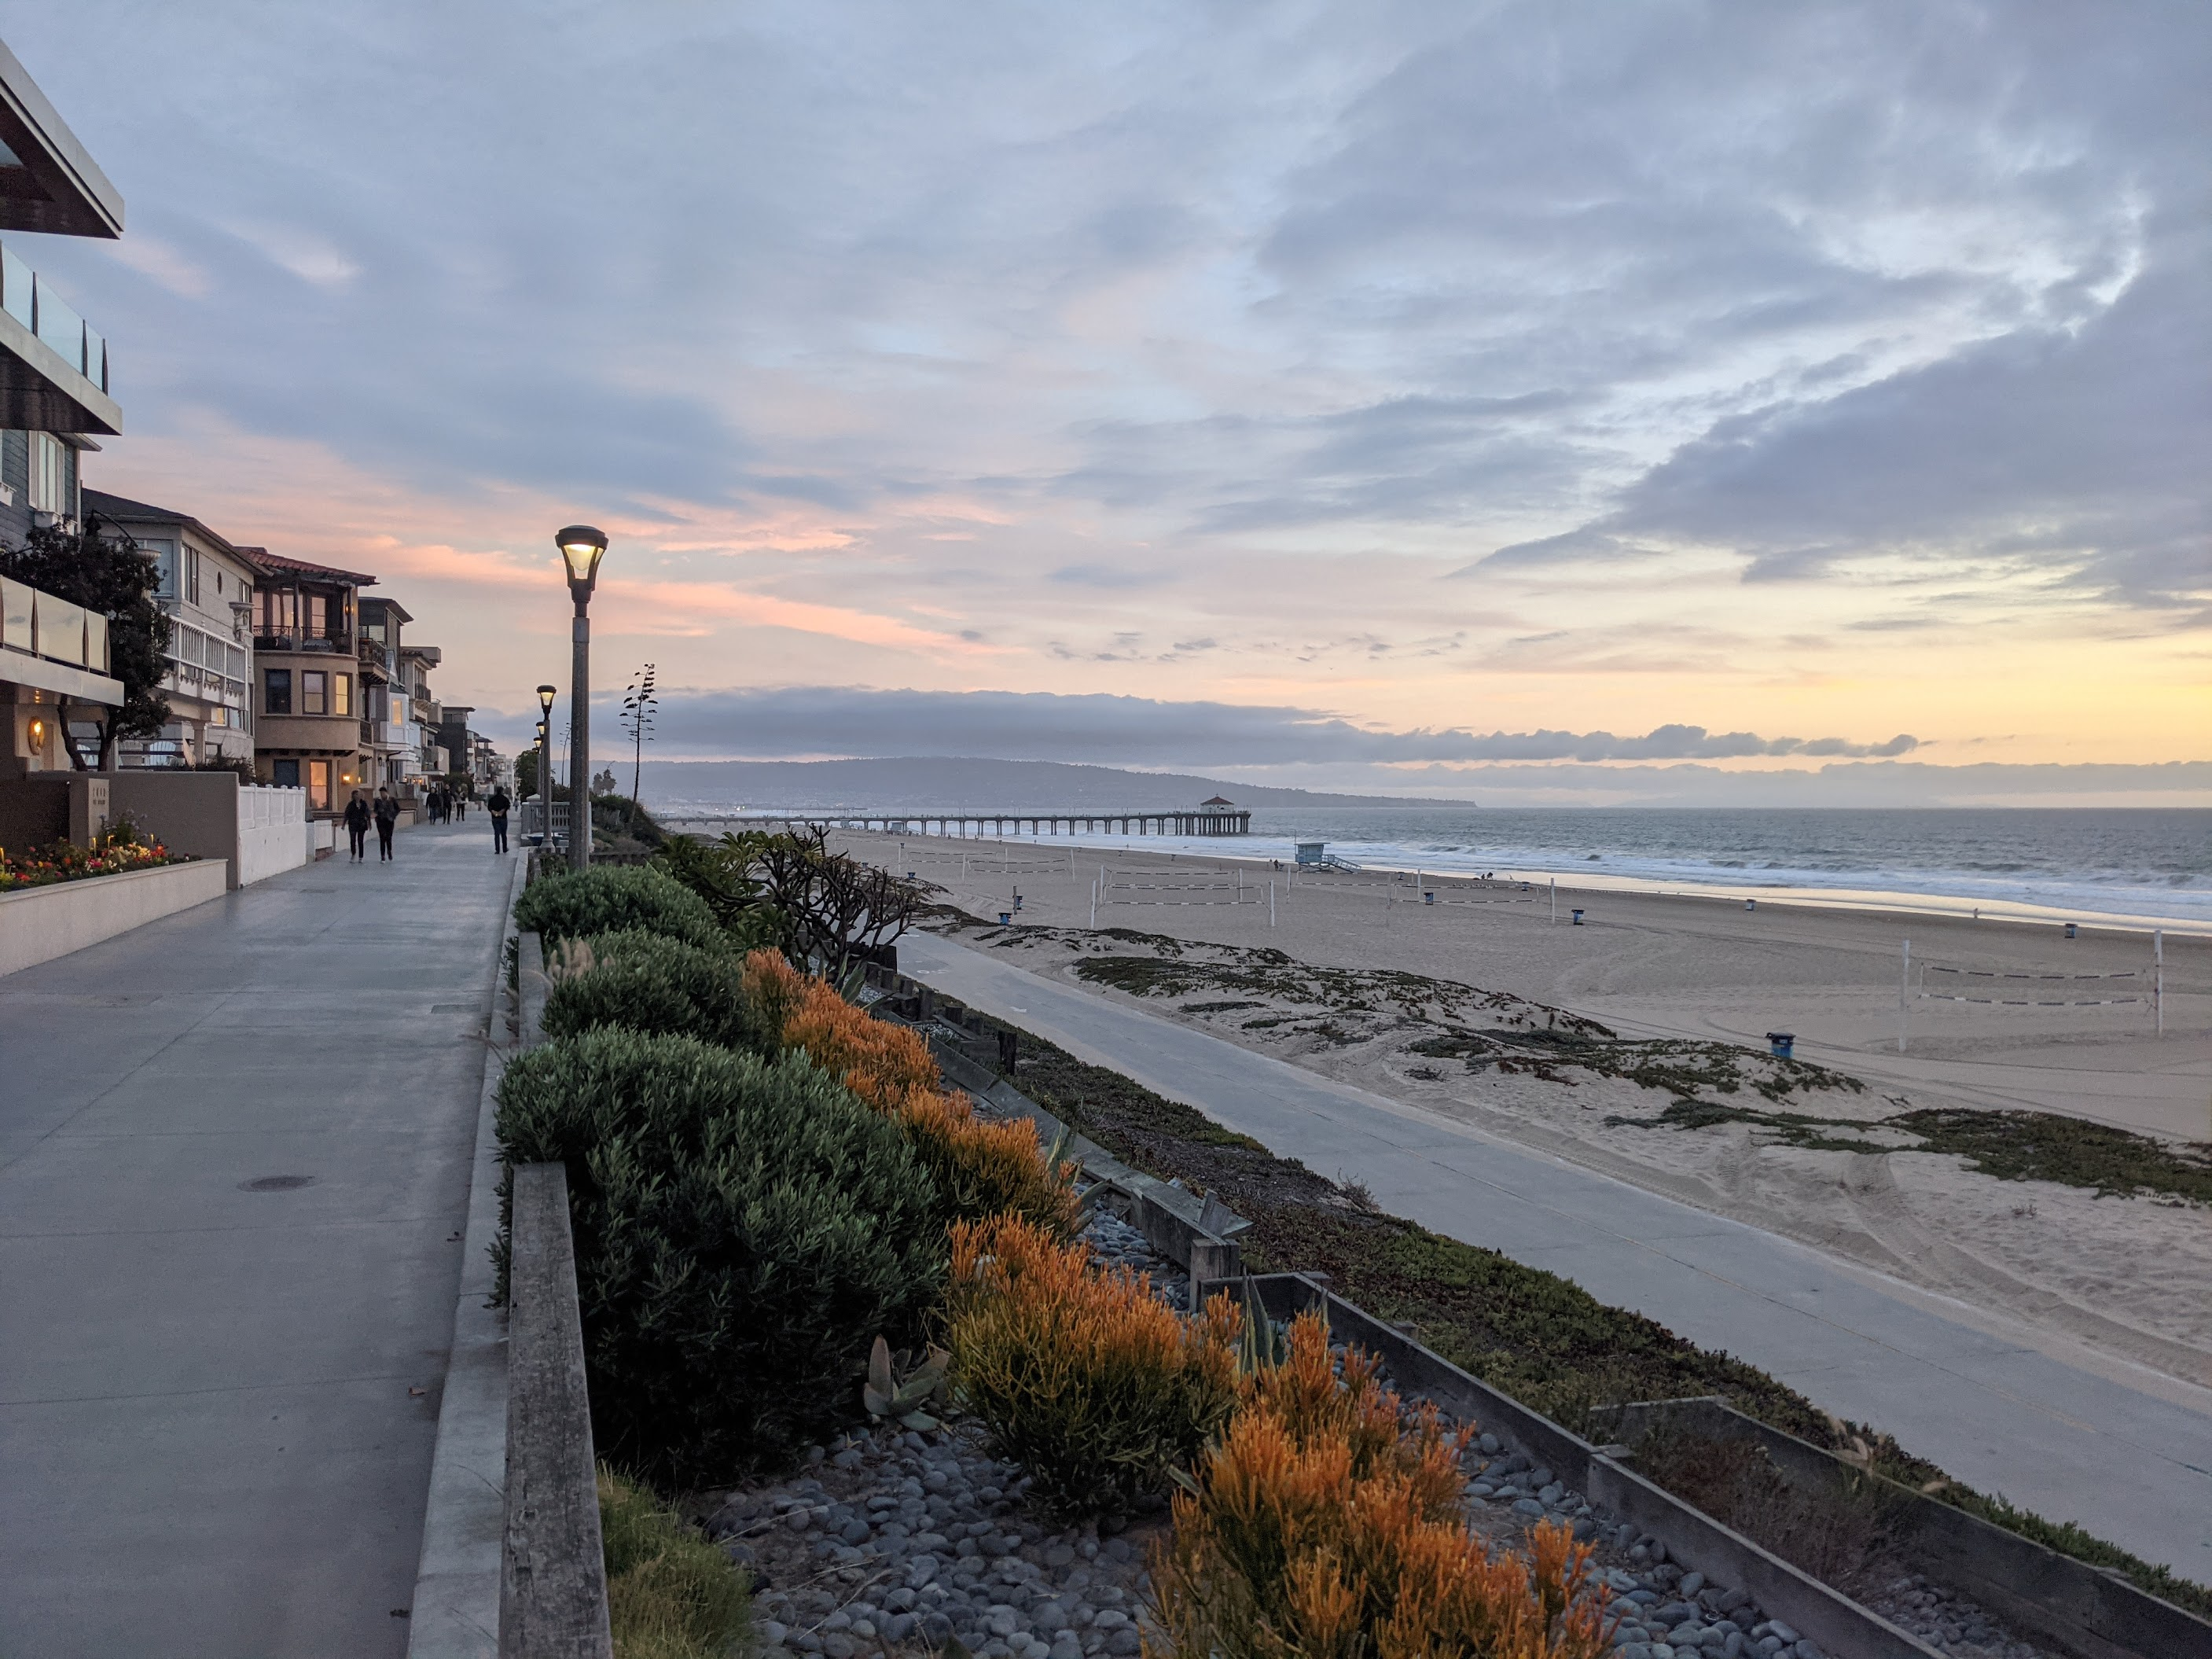
\includegraphics[width = \textwidth]{figures/mb3}\\
Source: Own photo
\end{frame}

\begin{frame}
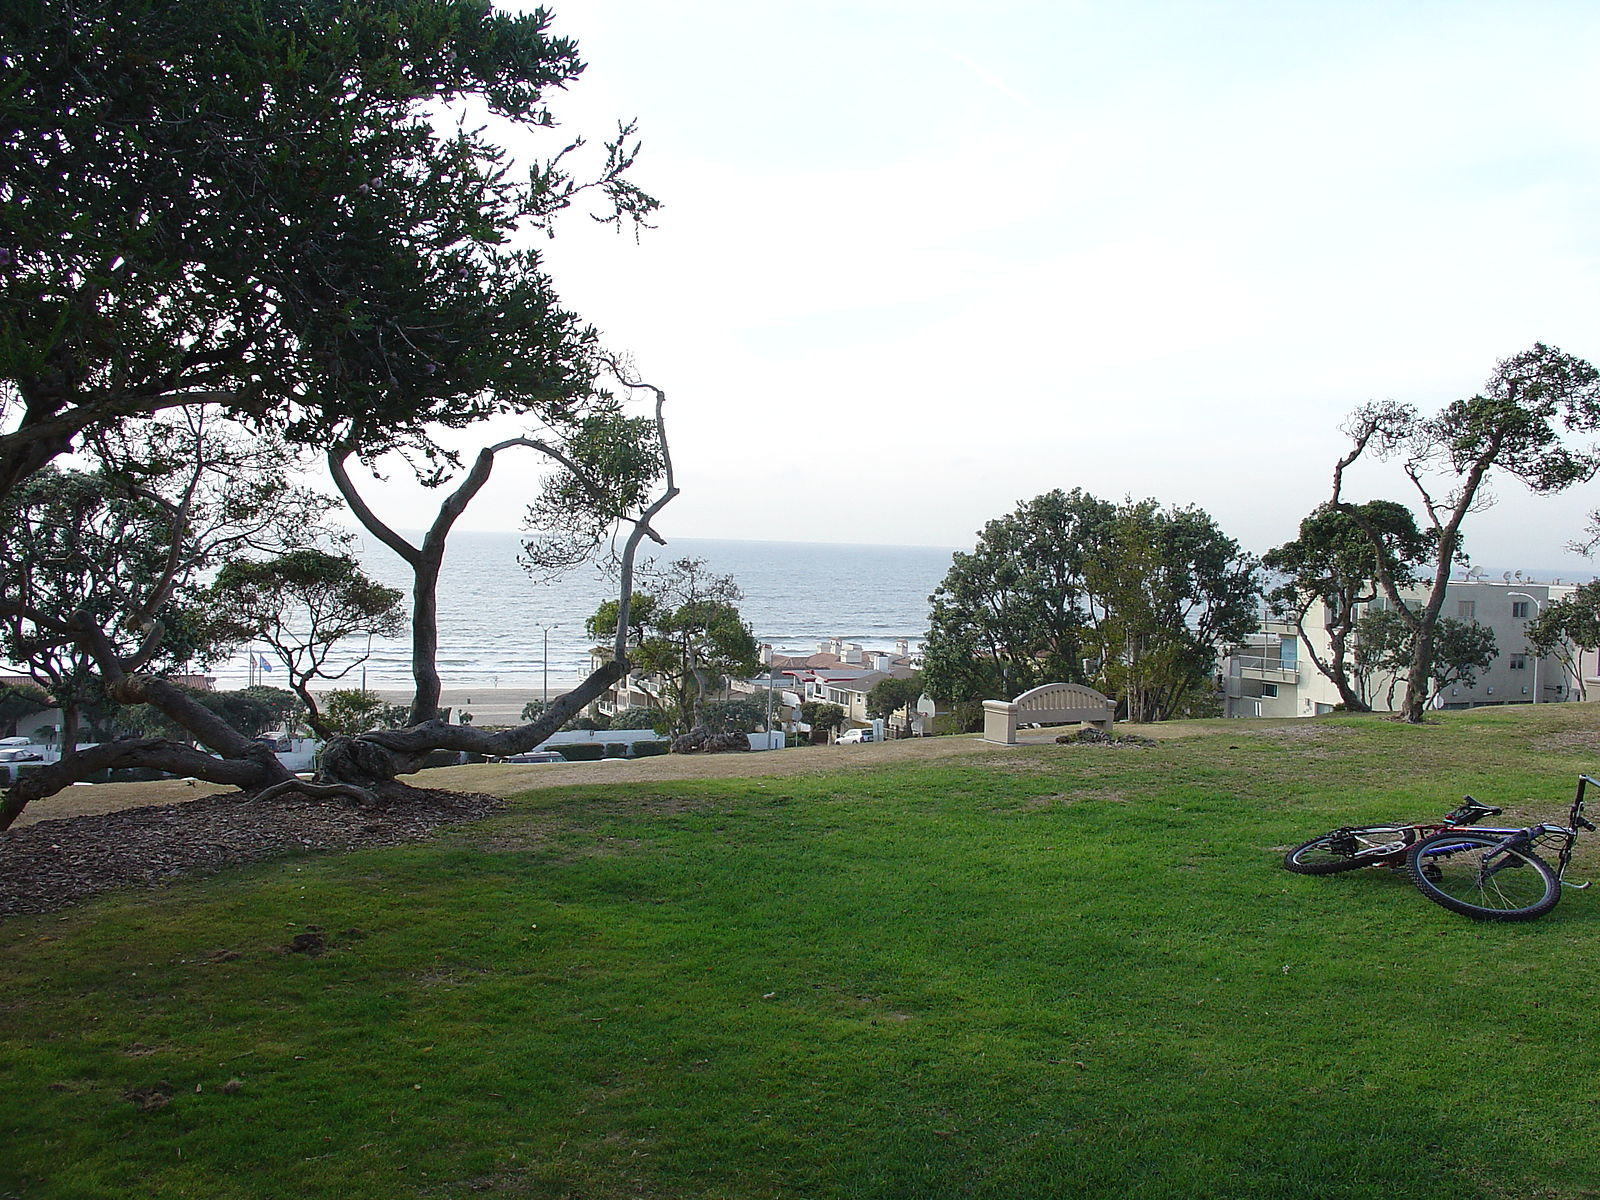
\includegraphics[width = \textwidth]{figures/park}\\
Source: Wikimedia
\end{frame}

\begin{frame}
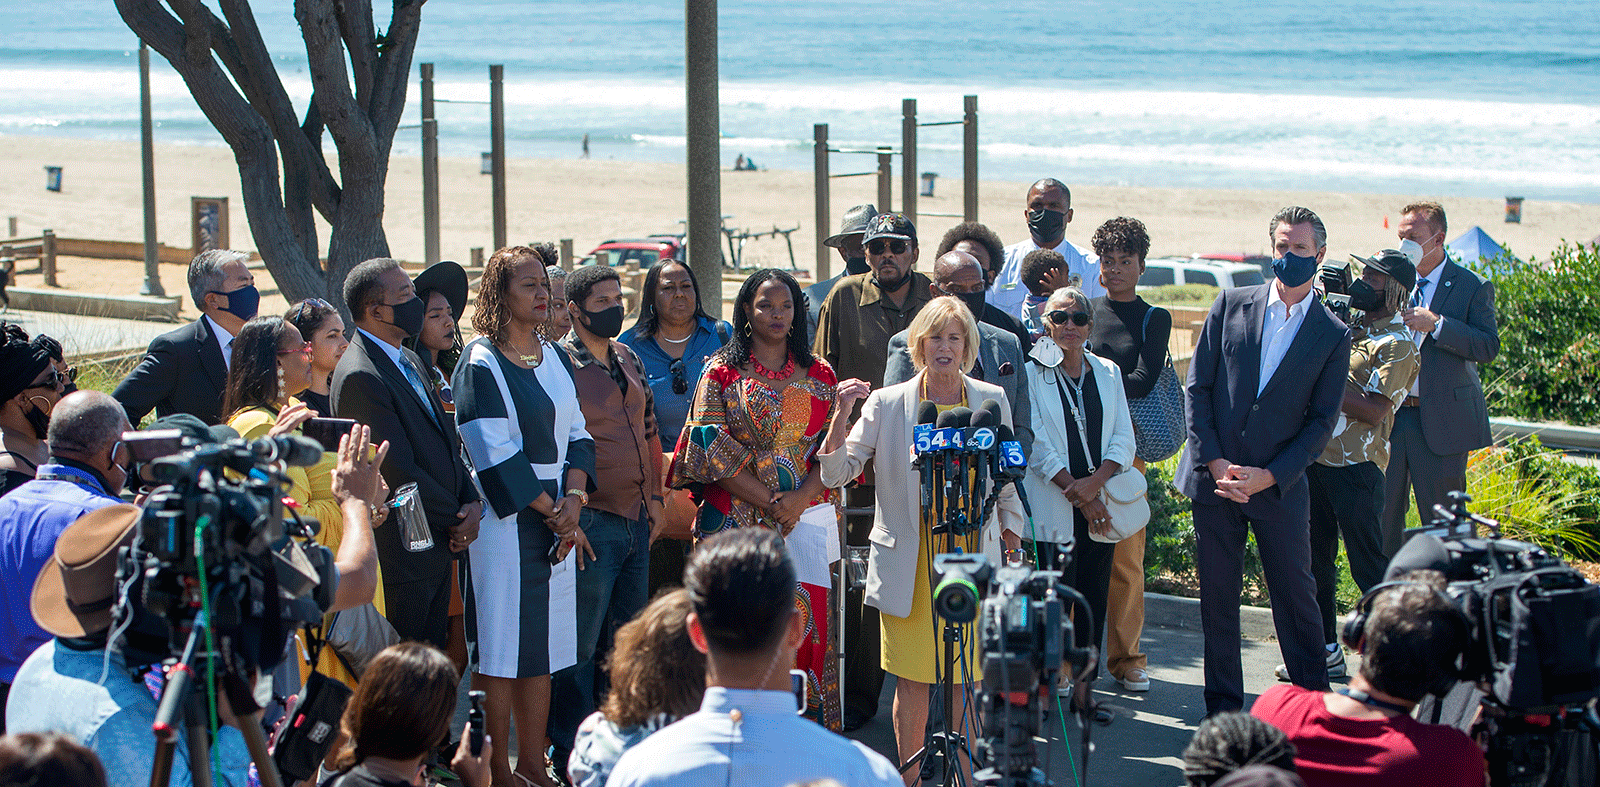
\includegraphics[width = \textwidth]{figures/reparation} \\
Source: \href{https://ceo.lacounty.gov/ardi/bruces-beach/}{County of Los Angeles}
\end{frame}

\begin{frame}{Discussion}
React
\begin{itemize}
\item What surprised you?
\item What resonated with you?
\item What questions does this raise for you?
\end{itemize}
\end{frame}

\begin{frame}{Discussion}
If you can inherit generational wealth, you can inherit generational debt. That’s debt that Manhattan Beach owes to the Bruce family. It’s debt that California and this nation owes to many more families like the Bruces. \vskip .1in
--- California State Senator Steve Bradford
\end{frame}

\begin{frame}{Discussion}
\begin{itemize}
\item What might Nozick say about this story?
\item What might Rawls have to say about this story?
\end{itemize}
\end{frame}

\begin{frame}{Discussion}
What role might research play in the debate about reparations?
\end{frame}

\begin{frame}
\Large
Land dispossession happens elsewhere, too \pause \vskip .2in
Including at Cornell
\end{frame}

\begin{frame}
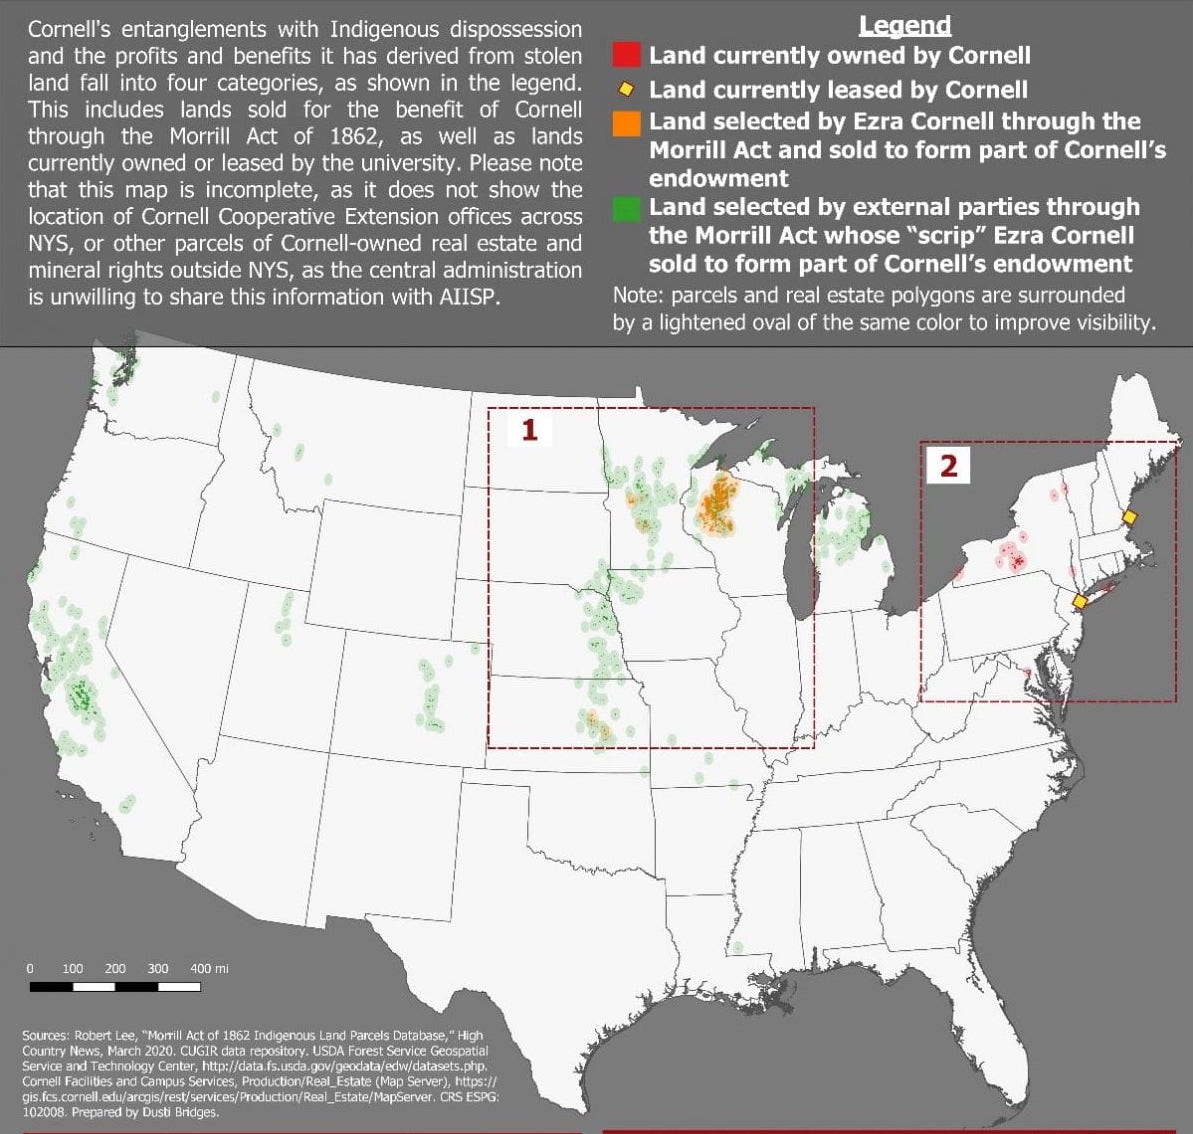
\includegraphics[width = \textwidth]{figures/cornell_dispossession}
\end{frame}

\begin{frame}

\includegraphics[width = .5\textwidth]{figures/cornell_dispossession_website} \\
\bref{https://blogs.cornell.edu/cornelluniversityindigenousdispossession/}{blogs.cornell.edu/cornelluniversityindigenousdispossession/}
\end{frame}

\begin{frame}
Supplemental
\end{frame}

\begin{frame}
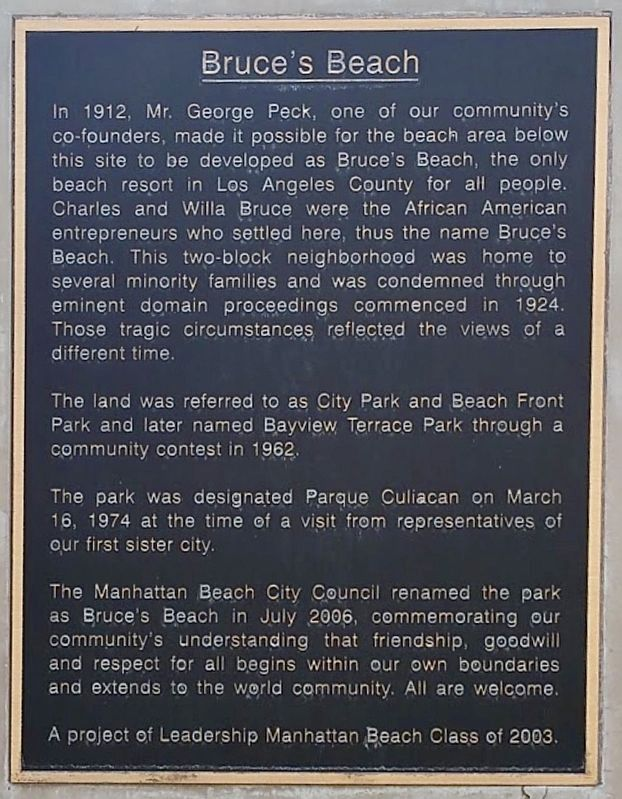
\includegraphics[width = \textwidth]{figures/plaque} \\
Source: Craig Baker via [The Historical Marker Databaset](https://www.hmdb.org/m.asp?m=170564)
\end{frame}

\end{document}

